Een diode\index{Diode} laat stroom door in \'e\'en richting, alleen van de anode (A) naar de kathode (C). Van de kathode naar de anode kan er geen stroom lopen.

In de elektronica wordt een diode weergegeven met het symbool dat je ziet weergegeven in \ref{symbool:diode}

\begin{figure}[h]
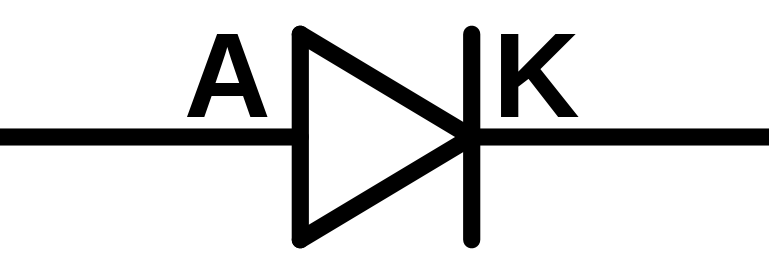
\includegraphics[width=5cm]{diode}
\centering
\caption{Symbool van een diode}
\label{symbool:diode}
\end{figure}

Een diode die licht kan geven noemen we een LED, Light Emitting Diode.
